
%% bare_conf.tex 
%% V1.2
%% 2002/11/18
%% by Michael Shell
%% mshell@ece.gatech.edu
%% 
%% NOTE: This text file uses MS Windows line feed conventions. When (human)
%% reading this file on other platforms, you may have to use a text
%% editor that can handle lines terminated by the MS Windows line feed
%% characters (0x0D 0x0A).
%% 
%% This is a skeleton file demonstrating the use of IEEEtran.cls 
%% (requires IEEEtran.cls version 1.6b or later) with an IEEE conference paper.
%% 
%% Support sites:
%% http://www.ieee.org
%% and/or
%% http://www.ctan.org/tex-archive/macros/latex/contrib/supported/IEEEtran/ 
%%
%% This code is offered as-is - no warranty - user assumes all risk.
%% Free to use, distribute and modify.

% *** Authors should verify (and, if needed, correct) their LaTeX system  ***
% *** with the testflow diagnostic prior to trusting their LaTeX platform ***
% *** with production work. IEEE's font choices can trigger bugs that do  ***
% *** not appear when using other class files.                            ***
% Testflow can be obtained at:
% http://www.ctan.org/tex-archive/macros/latex/contrib/supported/IEEEtran/testflow


% Note that the a4paper option is mainly intended so that authors in
% countries using A4 can easily print to A4 and see how their papers will
% look in print. Authors are encouraged to use U.S. letter paper when 
% submitting to IEEE. Use the testflow package mentioned above to verify
% correct handling of both paper sizes by the author's LaTeX system.
%
% Also note that the "draftcls" or "draftclsnofoot", not "draft", option
% should be used if it is desired that the figures are to be displayed in
% draft mode.
%
% This paper can be formatted using the peerreviewca
% (instead of conference) mode.
\documentclass[conference]{IEEEtran}
% If the IEEEtran.cls has not been installed into the LaTeX system files, 
% manually specify the path to it:
% \documentclass[conference]{../sty/IEEEtran} 


% some very useful LaTeX packages include:

%\usepackage{cite}      % Written by Donald Arseneau
                        % V1.6 and later of IEEEtran pre-defines the format
                        % of the cite.sty package \cite{} output to follow
                        % that of IEEE. Loading the cite package will
                        % result in citation numbers being automatically
                        % sorted and properly "ranged". i.e.,
                        % [1], [9], [2], [7], [5], [6]
                        % (without using cite.sty)
                        % will become:
                        % [1], [2], [5]--[7], [9] (using cite.sty)
                        % cite.sty's \cite will automatically add leading
                        % space, if needed. Use cite.sty's noadjust option
                        % (cite.sty V3.8 and later) if you want to turn this
                        % off. cite.sty is already installed on most LaTeX
                        % systems. The latest version can be obtained at:
                        % http://www.ctan.org/tex-archive/macros/latex/contrib/supported/cite/

%\usepackage{graphicx}  % Written by David Carlisle and Sebastian Rahtz
                        % Required if you want graphics, photos, etc.
                        % graphicx.sty is already installed on most LaTeX
                        % systems. The latest version and documentation can
                        % be obtained at:
                        % http://www.ctan.org/tex-archive/macros/latex/required/graphics/
                        % Another good source of documentation is "Using
                        % Imported Graphics in LaTeX2e" by Keith Reckdahl
                        % which can be found as esplatex.ps and epslatex.pdf
                        % at: http://www.ctan.org/tex-archive/info/
% NOTE: for dual use with latex and pdflatex, instead load graphicx like:
%\ifx\pdfoutput\undefined
%\usepackage{graphicx}
%\else
%\usepackage[pdftex]{graphicx}
%\fi

% However, be warned that pdflatex will require graphics to be in PDF
% (not EPS) format and will preclude the use of PostScript based LaTeX
% packages such as psfrag.sty and pstricks.sty. IEEE conferences typically
% allow PDF graphics (and hence pdfLaTeX). However, IEEE journals do not
% (yet) allow image formats other than EPS or TIFF. Therefore, authors of
% journal papers should use traditional LaTeX with EPS graphics.
%
% The path(s) to the graphics files can also be declared: e.g.,
% \graphicspath{{../eps/}{../ps/}}
% if the graphics files are not located in the same directory as the
% .tex file. This can be done in each branch of the conditional above
% (after graphicx is loaded) to handle the EPS and PDF cases separately.
% In this way, full path information will not have to be specified in
% each \includegraphics command.
%
% Note that, when switching from latex to pdflatex and vice-versa, the new
% compiler will have to be run twice to clear some warnings.


%\usepackage{psfrag}    % Written by Craig Barratt, Michael C. Grant,
                        % and David Carlisle
                        % This package allows you to substitute LaTeX
                        % commands for text in imported EPS graphic files.
                        % In this way, LaTeX symbols can be placed into
                        % graphics that have been generated by other
                        % applications. You must use latex->dvips->ps2pdf
                        % workflow (not direct pdf output from pdflatex) if
                        % you wish to use this capability because it works
                        % via some PostScript tricks. Alternatively, the
                        % graphics could be processed as separate files via
                        % psfrag and dvips, then converted to PDF for
                        % inclusion in the main file which uses pdflatex.
                        % Docs are in "The PSfrag System" by Michael C. Grant
                        % and David Carlisle. There is also some information 
                        % about using psfrag in "Using Imported Graphics in
                        % LaTeX2e" by Keith Reckdahl which documents the
                        % graphicx package (see above). The psfrag package
                        % and documentation can be obtained at:
                        % http://www.ctan.org/tex-archive/macros/latex/contrib/supported/psfrag/

%\usepackage{subfigure} % Written by Steven Douglas Cochran
                        % This package makes it easy to put subfigures
                        % in your figures. i.e., "figure 1a and 1b"
                        % Docs are in "Using Imported Graphics in LaTeX2e"
                        % by Keith Reckdahl which also documents the graphicx
                        % package (see above). subfigure.sty is already
                        % installed on most LaTeX systems. The latest version
                        % and documentation can be obtained at:
                        % http://www.ctan.org/tex-archive/macros/latex/contrib/supported/subfigure/

%\usepackage{url}       % Written by Donald Arseneau
                        % Provides better support for handling and breaking
                        % URLs. url.sty is already installed on most LaTeX
                        % systems. The latest version can be obtained at:
                        % http://www.ctan.org/tex-archive/macros/latex/contrib/other/misc/
                        % Read the url.sty source comments for usage information.

%\usepackage{stfloats}  % Written by Sigitas Tolusis
                        % Gives LaTeX2e the ability to do double column
                        % floats at the bottom of the page as well as the top.
                        % (e.g., "\begin{figure*}[!b]" is not normally
                        % possible in LaTeX2e). This is an invasive package
                        % which rewrites many portions of the LaTeX2e output
                        % routines. It may not work with other packages that
                        % modify the LaTeX2e output routine and/or with other
                        % versions of LaTeX. The latest version and
                        % documentation can be obtained at:
                        % http://www.ctan.org/tex-archive/macros/latex/contrib/supported/sttools/
                        % Documentation is contained in the stfloats.sty
                        % comments as well as in the presfull.pdf file.
                        % Do not use the stfloats baselinefloat ability as
                        % IEEE does not allow \baselineskip to stretch.
                        % Authors submitting work to the IEEE should note
                        % that IEEE rarely uses double column equations and
                        % that authors should try to avoid such use.
                        % Do not be tempted to use the cuted.sty or
                        % midfloat.sty package (by the same author) as IEEE
                        % does not format its papers in such ways.

%\usepackage{amsmath}   % From the American Mathematical Society
                        % A popular package that provides many helpful commands
                        % for dealing with mathematics. Note that the AMSmath
                        % package sets \interdisplaylinepenalty to 10000 thus
                        % preventing page breaks from occurring within multiline
                        % equations. Use:
%\interdisplaylinepenalty=2500
                        % after loading amsmath to restore such page breaks
                        % as IEEEtran.cls normally does. amsmath.sty is already
                        % installed on most LaTeX systems. The latest version
                        % and documentation can be obtained at:
                        % http://www.ctan.org/tex-archive/macros/latex/required/amslatex/math/

\usepackage[spanish]{babel}
%\usepackage[T1]{fontenc} %Paquetes de Fuentes que queramos usar
\usepackage[utf8]{inputenc}
%\usepackage[spanish]{babel}
\usepackage{amsmath,amssymb,amsfonts}
%\usepackage{fancyhdr}
\usepackage{graphicx} % Imagenes 
\usepackage{cite} 
\usepackage{hhline}
\usepackage{multicol}
\usepackage{longtable}
\usepackage{amssymb}
\usepackage{t1enc}
%\usepackage[letterpaper, left=3cm, right=2cm, top=2cm, bottom=2cm]{geometry} 
\usepackage{amsmath}
\usepackage{color}
%\usepackage[export]{adjustbox}
\usepackage{pdfpages}
\usepackage{subcaption}
\usepackage{hyperref}
\usepackage{listings}
\usepackage{float}
\usepackage{url}
\usepackage{textcomp}

% Other popular packages for formatting tables and equations include:

%\usepackage{array}
% Frank Mittelbach's and David Carlisle's array.sty which improves the
% LaTeX2e array and tabular environments to provide better appearances and
% additional user controls. array.sty is already installed on most systems.
% The latest version and documentation can be obtained at:
% http://www.ctan.org/tex-archive/macros/latex/required/tools/

% Mark Wooding's extremely powerful MDW tools, especially mdwmath.sty and
% mdwtab.sty which are used to format equations and tables, respectively.
% The MDWtools set is already installed on most LaTeX systems. The lastest
% version and documentation is available at:
% http://www.ctan.org/tex-archive/macros/latex/contrib/supported/mdwtools/


% V1.6 of IEEEtran contains the IEEEeqnarray family of commands that can
% be used to generate multiline equations as well as matrices, tables, etc.


% Also of notable interest:

% Scott Pakin's eqparbox package for creating (automatically sized) equal
% width boxes. Available:
% http://www.ctan.org/tex-archive/macros/latex/contrib/supported/eqparbox/



% Notes on hyperref:
% IEEEtran.cls attempts to be compliant with the hyperref package, written
% by Heiko Oberdiek and Sebastian Rahtz, which provides hyperlinks within
% a document as well as an index for PDF files (produced via pdflatex).
% However, it is a tad difficult to properly interface LaTeX classes and
% packages with this (necessarily) complex and invasive package. It is
% recommended that hyperref not be used for work that is to be submitted
% to the IEEE. Users who wish to use hyperref *must* ensure that their
% hyperref version is 6.72u or later *and* IEEEtran.cls is version 1.6b 
% or later. The latest version of hyperref can be obtained at:
%
% http://www.ctan.org/tex-archive/macros/latex/contrib/supported/hyperref/
%
% Also, be aware that cite.sty (as of version 3.9, 11/2001) and hyperref.sty
% (as of version 6.72t, 2002/07/25) do not work optimally together.
% To mediate the differences between these two packages, IEEEtran.cls, as
% of v1.6b, predefines a command that fools hyperref into thinking that
% the natbib package is being used - causing it not to modify the existing
% citation commands, and allowing cite.sty to operate as normal. However,
% as a result, citation numbers will not be hyperlinked. Another side effect
% of this approach is that the natbib.sty package will not properly load
% under IEEEtran.cls. However, current versions of natbib are not capable
% of compressing and sorting citation numbers in IEEE's style - so this
% should not be an issue. If, for some strange reason, the user wants to
% load natbib.sty under IEEEtran.cls, the following code must be placed
% before natbib.sty can be loaded:
%
% \makeatletter
% \let\NAT@parse\undefined
% \makeatother
%
% Hyperref should be loaded differently depending on whether pdflatex
% or traditional latex is being used:
%
%\ifx\pdfoutput\undefined
%\usepackage[hypertex]{hyperref}
%\else
%\usepackage[pdftex,hypertexnames=false]{hyperref}
%\fi
%
% Pdflatex produces superior hyperref results and is the recommended
% compiler for such use.



% *** Do not adjust lengths that control margins, column widths, etc. ***
% *** Do not use packages that alter fonts (such as pslatex).         ***
% There should be no need to do such things with IEEEtran.cls V1.6 and later.


% correct bad hyphenation here
%\hyphenation{op-tical net-works semi-conduc-tor IEEEtran}
\newtheorem{definition}{Definici\'on}
\newcommand{\rand}{\stackrel{\$}\leftarrow}

\begin{document}

% paper title
\title{Aplicación de cifrado contra adversarios clasificadores, para el correo electrónico}


% author names and affiliations
% use a multiple column layout for up to three different
% affiliations
%\author{\authorblockN{Michael Shell}
%\authorblockA{School of Electrical and\\Computer Engineering\\
%Georgia Institute of Technology\\
%Atlanta, Georgia 30332--0250\\
%Email: mshell@ece.gatech.edu}
%\and
%\authorblockN{Homer Simpson}
%\authorblockA{Twentieth Century Fox\\
%Springfield, USA\\
%Email: homer@thesimpsons.com}
%}


% avoiding spaces at the end of the author lines is not a problem with
% conference papers because we don't use \thanks or \IEEEmembership


% for over three affiliations, or if they all won't fit within the width
% of the page, use this alternative format:
% 
\author{\authorblockN{Jonathan Arcos Ayala\authorrefmark{1},
Allan U. Zepeda Ibarra\authorrefmark{2}, Sandra D\'iaz Santiago\authorrefmark{3} y Manuel A. Soto Ramos\authorrefmark{4}}
\authorblockA{Escuela Superior de Cómputo,
Instituto Politécnico Nacional\\
Ciudad de México.\\ Tel.57-29-6000 ext.52022} 
\authorblockA{Email: \authorrefmark{1}jonas.arc.99@gmail.com, \authorrefmark{2} balaju01@gmail.com,\authorrefmark{3}sdiazsa@ipn.mx, \authorrefmark{4}msotoa06@yahoo.com.mx}
}



% use only for invited papers
%\specialpapernotice{(Invited Paper)}

% make the title area
\maketitle

\begin{abstract}
En este Trabajo Terminal se desarroll\'o una herramienta de cifrado que protege al correo electrónico, contra un tipo especial de adversario, denominado adversario clasificador. El objetivo de este adversario es analizar una gran cantidad de información, para clasificar al usuario en categorías predeterminadas. La herramienta que se propone utiliza de manera novedosa los CAPTCHAs y una técnica criptográfica conocida como secreto compartido, para facilitar el acuerdo de las claves de cifrado. Adicionalmente, la aplicación utilizará un servidor de llaves para la autenticación de los usuarios para proveer una forma segura de enviar mensajes cifrados y recuperarlos.
\end{abstract}


%\keywords{Criptograf\'ia, Correo electr\'onico, Secreto compartido, CAPTCHAs.}
% no keywords

% For peer review papers, you can put extra information on the cover
% page as needed:
% \begin{center} \bfseries EDICS Category: 3-BBND \end{center}
%
% for peerreview papers, inserts a page break and creates the second title.
% Will be ignored for other modes.
%\IEEEpeerreviewmaketitle



\section{Introducci\'on}
% no \PARstart
Actualmente, una gran cantidad de personas hacen uso del internet y de las nuevas tecnologías para comunicarse. Con ello, también se incrementa la cantidad de información que se transmite y/o almacena. En diversas ocasiones, esta información es susceptible a sufrir distintos tipos de ataques, tales como acceso no autorizado, modificación o destrucción de la misma, entre otros. Adicionalmente, cada día aparecen nuevos tipos de ataques a los sistemas de información. Por lo tanto, surge la necesidad de proteger dicha información.\\
Una de las tecnologías ampliamente usada para comunicarse es el correo electrónico \cite{@}. Los mensajes que envían y reciben los usuarios de correo electrónico pueden ser de diferentes tipos: personales, transaccionales, de notificación o de publicidad. Por lo tanto, cada vez que se escribe y envía un correo electrónico, se está revelando información acerca de las preferencias y/o intereses del usuario. Estos datos, son el insumo más importante, para distintas entidades, entre las cuales están empresas que realizan publicidad en línea, proveedores de internet, instituciones de gobierno, entre otros \cite{sp}.
El propósito de tener estos datos puede ser realizar publicidad efectiva, vender los datos a empresas de publicidad o averiguar si determinado usuario es una amenaza para el gobierno. Para obtener información acerca de los intereses y/o preferencias del usuario, se hace uso de programas de cómputo denominados \textit{clasificadores}. Los clasificadores son herramientas informáticas que analizan una gran cantidad de información, haciendo uso de técnicas de aprendizaje máquina \cite{stanford}, y posteriormente clasifican un mensaje en determinada categoría o perfil. 
En este contexto, los clasificadores pueden constituir una amenaza para algunos usuarios del correo electrónico, por tal motivo de ahora en adelante a los programas que clasifican se les denominará \textit{adversarios clasificadores}.\\
Ante tal escenario, surge la pregunta ¿cómo se puede proteger un usuario contra los adversarios clasificadores? Una posible respuesta es hacer uso de algoritmos de cifrado estándar. Sin embargo, hacer uso de tales algoritmos, implica que los participantes en la comunicación acuerden una clave de cifrado. Desafortunadamente, acordar una clave, no es un proceso sencillo para el usuario común. Otra desventaja de esta primera solución, es que los algoritmos de cifrado estándar ofrecen un alto nivel de seguridad, el cual resulta excesivo cuando se consideran los recursos y el objetivo de un adversario clasificador~\cite{clas}.
%La  única  referencia  que se tiene  sobre  un  esquema  criptográfico  contra  adversarios clasificadores es el que propusieron Golle y Farahat~\cite{Attacks}. En este art\'iculo se habla por primera vez de las caracter\'isticas de este tipo de adversarios  y se considera la posibilidad de utilizar un esquema de cifrado con un nivel de seguridad menor.
%en el artículo 
%“Defending Email Communication Against Profiling” de Philippe Golle  y  Ayman  Farahat, ambos  miembros del 
%“Palo Alto Research Center”.\cite{Attacks}\\
%En su artículo se aborda el ataque de adversarios clasificadores sobre los mensajes de correo electrónico, en el cual se proponen un protocolo para la comunicación por correo electrónico. 

Una soluci\'on alternativa fue presentada por Golle y Farahat~\cite{Attacks} quienes proponen un protocolo que hace uso de una función  de cifrado, el cual sustituye cada una de las palabras del mensaje por otra de la misma extensión y frecuencia gramatical, esta función esta pensada para textos en idioma ingl\'es. 
%Esta función tiene como parámetro una clave $K$.  
Para cifrar se utiliza una clave que se genera  usando los datos de cabecera que acompañan al mensaje los cuales pueden ser dirección  del remitente, la dirección del destinatario, la hora a la que se envía el correo electrónico y potencialmente otros campos. Estos datos se introducen en una función hash lenta y el resultado de esta función es la clave $K$. Estas funciones hash  tiene con una complejidad de c\'alculo moderadamente mas alta que las 
funciones hash est\'andar.  \\
Este  protocolo resulta inseguro para la criptografía moderna pero es efectivo contra el ataque de clasificadores. Por otro lado este protocolo resuelve dos problemas, le  permite  a los usuarios  calcular  la  clave de cifrado y descifrado  fácilmente  ya  que  los datos del mensaje con que se calcula son  públicos, resolviendo así el intercambio de claves. Al usar un cifrado de tipo semántico se permite que el texto se vea como un texto en inglés pero indistinguible para los clasificadores y por lo tanto este clasifica incorrectamente el mensaje cifrado.

D\'iaz y Chakraborty~\cite{clas} propusieron un nuevo esquema que no requiere de un intercambio previo de claves, 
ni de una infraestructura de clave p\'ublica.  Puesto que un adversario en cuesti\'on es un programa de c\'omputo, tal esquema utiliza CAPTCHAs para esconder la clave de cifrado. Este esquema es el que se implement\'o en el presente trabajo. 

El resto del art\'iculo est\'a organizado como sigue, en la Secci\'on~\ref{sec-prelim} se presentan los conceptos b\'asicos asociados con criptograf\'ia, en la Secci\'on~\ref{sec-esquemaDC} se describe el esquema propuesto por D\'iaz y Chakraborty,
en la Secci\'on~\ref{sec-implem} se muestran los detalles de la implementaci\'on y finalmente en la Secci\'on~\ref{sec-conclusion} se presentan las conclusiones.

%\hfill mds
 
%\hfill Junio 07, 2016

%\section{Adversarios Clasificadores}
%Los adversarios clasificadores son programas de c\'omputo que se dedican a observar  mensajes que se intercambian  entre  los  usuarios  de  correo  electrónico,  con  el  fin  de  clasificarlos  e 
%identificar  a  todos  los  usuarios  que  cumplan  con  cierto  criterio.  Esta  clasificación  se hace de manera masiva a trav\'es de  una búsqueda de palabras clave dentro de 
%los  mensajes de  los usuarios. Por ejemplo, el  clasificador puede estar interesado en  los mensajes  que  contienen  la  palabra  clave  "Bomba",  así  que 
%todos  los  mensajes  que contengan esta palabra serán etiquetados en una clasificación en específico, este proceso se lleva a cabo por medio de técnicas de 
%“Reconocimiento de patrones” y “Aprendizaje Máquina” para encontrar y clasificar los mensajes 
%que intercepta~\cite{clas,Attacks}.
%\\
%La  clasificación  de  estos  mensajes  tiene  diversos  usos, ya  que  pueden  ser  clasificados con  fines demográficos, con  fines comerciales o con  fines gubernamentales. Todo esto 
%con  el  propósito  de  generar  las  estadísticas  de  comportamientos  e  intereses  de  los usuarios de correo electrónico. \\
%
%
%
%
%En este trabajo terminal, se considera que un adversario clasificador solo es capaz de realizar ataques de texto cifrado (ciphertext only attack, en ingl\'es). Como se mencion\'o en el cap\'itulo anterior, en este ataque  el adversario solo  cuenta  con  los  textos  cifrados  que  va  recopilando  de  un  canal  o  base  de 
%datos. Posteriormente, el adversario utiliza  estos  textos  cifrados  para  hacer  un  análisis  criptográfico  de  cómo  se comporta la técnica de cifrado  y tratar de hallar el texto en claro a partir de los textos cifrados que va recopilando. 
%\\
%Este  tipo  de  ataques  es  muy  común  en  el  internet  aunque  con  muy  baja  efectividad cuando   se   implementa   en   comunicaciones   altamente   protegidas,   y   cuando   se 
%implementa en canales de comunicación desprotegidos  la  información obtenida  llega  a ser  muy  pobre.  En  los  últimos  años  se  han  dado  cuenta  que  si   este  tipo  de 
%adversarios   atacan las  comunicaciones  sin  cifrado se  obtienen  características  valiosas  sobre  los usuarios  que  utilizan  este  tipo  de  canales  de  comunicación,  este  tipo  de  ataques  son 
%ejecutados por  adversarios clasificadores.\\
\section{Metodolog\'ia}
\subsection{Preliminares}
\label{sec-prelim}
\begin{definition} 
Un esquema de cifrado sim\'etrico est\'a conformado por una tripleta de algoritmos 
$\sf \Pi=(Gen, Enc, Dec)$, definidos como se describe a continuaci\'on:
\begin{itemize}
\item  El algoritmo generador de claves $\sf Gen$ selecciona una llave  $K$ al azar del conjunto de llaves $\cal K$, esto se denotar\'a como $K \rand {\cal K}$.
Esta clave $K$  ser\'a usada por los algoritmos  $\sf Enc$ y $\sf Dec$, esta clave la compartir\'an  emisor y receptor. 
\item El algoritmo de cifrado $\sf Enc$, toma como entrada un texto en claro  $M \in {\cal M}$ y una clave $K$ generada por  $\sf Gen$  y regresa un texto cifrado $C \in {\cal C}$.  Usualmente esto se denota como $C \leftarrow {\sf Enc}_K(M)$.
 \item El algoritmo de descifrado $\sf Dec$, toma como entrada un texto cifrado $C$ y una llave $K$ y regresa $M$. Esta operaci\'on se denota por  $M \leftarrow {\sf Dec}_K(C)$.
Para que cualquier algoritmo de cifrado sim\'etrico funcione correctamente, se debe garantizar que para
todas las llaves posibles en  $\cal K$ y todos los posibles mensajes $\cal M$, $$ {\sf Dec}_K({\sf Enc}_K(M)) = M.$$
\end{itemize}
\end{definition}
\begin{definition}
Una funci\'on hash, es una funci\'on de un s\'olo sentidocuya entrada $m$
 es un mensaje de longitud arbitraria
y la salida es una cadena binaria de longitud fija. Al resumen o hash de 
un mensaje $m$, se le denotar\'a como $H(m)$. Una funci\'on hash debe
tener las siguientes propiedades:
\begin{itemize}
\item Para cualquier mensaje $m$, debe ser posible calcular $H(m)$ 
eficientemente. 
\item Dado $H(m)$, debe ser computacionalmente dif\'icil, hallar un mensaje
$m'$, tal que $H(m)=H(m')$.
\item Debe ser computacionalmente dif\'icil, hallar dos mensajes $m$ y $m'$ 
tales que $H(m)=H(m')$.
\end{itemize}
\end{definition}


\subsubsection{Esquema de Secreto Compartido de Shamir}
El esquema de secreto compartido fue propuesto por Adi Shamir en 1997\cite{shamir}. 
El objetivo de este método es dividir un secreto $K$ en $w$ partes,que son dadas a $w$ participantes. Para recuperar el secreto es necesario tener al menos $u$
elementos de las $w$ partes siendo $u \leq w$. Y no es posible recuperar el secreto si se tienen menos que $u$ partes.

Para construir el esquema del secreto compartido primero es necesario seleccionar un número primo $p \geq w+1$ el cual define al conjunto $\mathbb{Z}_p$.
\\
\\
El procedimiento para dividir un secreto $K$ en $w$ partes es el siguiente:

\begin{enumerate}
 \item Se seleccionan $w$ elementos distintos de cero del conjunto $\mathbb{Z}_p$ denotados como $x_i$ donde $1 \leq i \leq w$.
 \item Se seleccionan $u-1$ elementos aleatorios de $\mathbb{Z}_p$ denotados como $a_1,...,a_{u-1}$.
 \item Se construye el polinomio $y_x$ de la siguiente forma. Sea \begin{equation}
            y(x)=K+\sum_{j=1}^{u-1} a_j x^j \bmod \quad p
           \end{equation}
           Por medio de este polinomio se calculan los elementos $y_i$.
 \item La salida es el conjunto $S=\{(x_1,y_1),...,(x_w,y_w)\}$.
\end{enumerate}

Para recuperar el secreto solo tenemos que resolver un sistema de ecuaciones  que es definido por el polinomio característico $a(x)=a_0+a_1x+...+a_{u-1}x^{u-1}$.
\\
\\
Posteriormente se seleccionan $u$ pares de elementos $(x_w,y_w)$ con los que obtendremos nuestro sistema de ecuaciones a resolver. 
%El elemento que nos interesa obtener del sistema de ecuaciones es $a_0$ ya que este es el valor de nuestro secreto $K$.

\subsubsection{CAPTCHA}
 Es un programa informático diseñado para diferenciar un ser humano de una computadora, CAPTCHA son las siglas de prueba de Turing completamente automática y pública para diferenciar computadoras de humanos ({\it Completely Automated Public Turing test to tell Computers and Humans Apart} por sus siglas en ingl\'es)~\cite{Ahn03}.  Un CAPTCHA es una prueba que es fácil de pasar por un usuario humano pero difícil de pasar por una máquina. Uno de los CAPTCHAs más com\'unes son imágenes distorsionadas de cadenas cortas de caracteres. Para un humano es generalmente muy fácil recuperar la cadena original de la imagen distorsionada, pero es difícil para  los algoritmos de reconocimiento de caracteres recuperar la cadena original de la imagen distorsionada.\\
Un CAPTCHA en un algoritmo aleatorio $G$, que recibe como parámetro una cadena de caracteres STR y produce como resultado un CAPTCHA $G(x)$\\


%\subsection{Polinomio de interpolación de Lagrange}
%
%\textbf{ejemplo}\\
%Si se considera el conjunto  $\mathbb{Z}_{11}$ y se desea compartir el secreto $K=8$, entre 5 participantes,
%de tal manera que solo cuando se re\'unan cualesquiera 2 de ellos sea posible recuperar $K$, es decir
% $w=5$ y $u=2$.
%
%Se seleccionan los $u-1$ elementos del conjunto $\mathbb{Z}_{11}$, puesto que $u=2$ en este caso solo 
%hay que escoger un elemento: $a_1=5$.
%
%A continuaci\'on se seleccionan $w$ elementos de $\mathbb{Z}_{11}$, por ejemplo 
% $x_1=2, x_2=7, x_3=9, x_4=10, x_5=3$.
%
%Posteriormente, se calcula el conjunto de elementos $y_i$ por medio de la ecuaci\'on 
%\begin{equation} \nonumber
% y_i=k+\sum_{j=1}^{u-1} a_j x_i^j \bmod \quad p
%\end{equation}
%
%En el caso del ejemplo, la ecuaci\'on anterior queda como sigue:
%
%\begin{equation} \nonumber
% y_i=K+a_1x_i \bmod \quad p
%\end{equation}
%Y se obtienen los siguientes valores:
%$$\begin{array}{lcl}
%y_1&=&8+5(2) \bmod 11=7, \\
%y_2&=&8+5(7) \bmod 11=10,\\
%y_3&=&8+5(9) \bmod 11=9, \\ 
%y_4&=&8+5(10) \bmod11=3, \\
%y_5&=&8+5(3) \bmod 11=1. 
%\end{array}$$
%
%Finalmente, se tienen los pares $S=\{ (2,7), (7,10), (9,9), (10,3),(3,1)\}$
%%$A_1(2,7)$\hspace{1cm}$A_2(7,10)$\hspace{1cm}$A_3(9,9)$\hspace{1cm}$A_4(10,3)$\hspace{1cm}$A_5(3,1)$\\
%
%
%Para recuperar la llave $K$ es necesario seleccionar $u=2$ pares del conjunto $S$, por ejemplo
%$A_2(7,10)$, $A_4(10,3)$. Con estos pares se puede crear el siguiente  sistema de ecuaciones:
%$$\begin{array}{lcl}
% a_0+a_1x_2&=&y_2 \\
% a_0+a_1x_4&=&y_4 
% \end{array}$$
% Es importante notar, que en tal sistema de ecuaciones, las inc\'ognitas son $a_0$ y $a_1$, las cuales
% son desconocidas para los $w$ participantes.  Para el esquema de secreto compartido de
% Shamir, es de particular inter\'es $a_0$, ya que  $a_0=K$.
%Al sustituir los pares $A_2$ y $A_4$ en el sistema de ecuaciones anterior, se tiene:
%\begin{align}
%a_0+7a_1&=10 \label{eq2-3}\\
%a_0+10a_1&=3 \label{eq2-4}
%\end{align}
%
%Para resolver este sistema se puede utilizar cualquiera de los métodos com\'unes que se usan en álgebra, solo que respetando el conjunto $\mathbb{Z}_p$, en este caso se resolverá por el polinomio de interpolación de Lagrange.
%\begin{equation}
% a_x=\sum_{j=1}^{u}y_i\prod\frac{x-x_j}{x_i-x_j} mod \quad p\label{eq2-5}
%\end{equation}
%
%Al sustituir los valor $A_2$ y $A_4$ en la ecuación anterior se puede calcular $a_0$. Pero una simplificación es posible, si se toma en cuenta que no es necesario conocer todo el polinomio, bastará con sólo deducir el termino $a_0$. Por lo tanto en la ecuación (\ref{eq2-5}) se sustituye $x=0$ quedando de la siguiente forma.
%\begin{equation}
% l_i=\prod\frac{-x_j}{x_i-x_j}\label{eq2-6}
%\end{equation}
%\begin{equation}
% a_0=\sum_{j=1}^{u}\hspace{0.1cm}y_i\hspace{0.1cm}l_i \hspace{0.1cm}mod \quad p\label{eq2-7}
%\end{equation}
%
%Sustituyendo el par $A_2$ en la ecuación (\ref{eq2-6}), se tiene:
%\\
%\begin{equation}
%l_2=\frac{-x_4}{x_2-x_4}=\frac{-10}{7-10}=\frac{-10}{-3}\hspace{0.1cm}mod\hspace{0.1cm}11=\frac{1}{8}\label{eq2-8}
%\end{equation}
%\\
%Se realiza la misma sustitución en la ecuación (\ref{eq2-6}) pero con el par $A_4$ dándonos como resultado:
%\\
%\begin{equation}
%l_4=\frac{-x_2}{x_4-x_2}=\frac{-7}{10-7}=\frac{-7}{3}\hspace{0.1cm}mod\hspace{0.1cm}11=\frac{4}{3}\label{eq2-9}
%\end{equation}
%\\
%Como la ecuación (\ref{eq2-7}) es una sumatoria podemos desarrollarla, dándonos como resultado: 
%\\
%\begin{equation}
%a_0=(y_2\hspace{0.1cm}l_2+y_4\hspace{0.1cm}l_4)\hspace{0.1cm}mod\hspace{0.1cm}11 
%\end{equation}
%\\
%realizamos la sustitución de $y_2$, $l_2$, $y_4$ y $l_4$.
%\\
%\begin{equation}
%a_0=(10\hspace{0.1cm}(\frac{1}{8})+3\hspace{0.1cm}(\frac{4}{3}))\hspace{0.1cm}mod\hspace{0.1cm}11 \label{eq2-10}
%\end{equation}
%\\
%Puesto que 7 es el inverso multiplicativo de 8 y 4 es el inverso multiplicativo de 3,  la ecuación~(\ref{eq2-10}) queda de la siguiente forma
%
%\begin{equation}
%a_0=((10)\hspace{0.1cm}(7)+(3)\hspace{0.1cm}(4))\hspace{0.1cm}mod\hspace{0.1cm}11 = 8
%\end{equation}
%
%Como $a_0=8$ podemos ver que se recuper\'o a $K$ exitosamente ya que  $a_0=K$.




\subsection{Esquema Díaz - Chakraborty}
\label{sec-esquemaDC}
El esquema D\'iaz-Chakraborty~\cite{clas} utiliza CAPTCHAs y un algoritmo de clave secreta,
para  proteger el correo electr\'onico. 
 Para obtener la clave se genera una cadena al azar, a la se le aplica una funci\'on hash, con esta clave se cifra el
 mensaje.  Tanto el mensaje cifrado como el CAPTCHA se env\'ian al receptor. El receptor debe
resolver el CAPTCHA, para obtener la cadena, aplicarle la funci\'on hash y as\'i obtener la clave de cifrado. Puesto que un adversario clasificador es un programa de c\'omputo, no podr\'a resolver un CAPTCHA y por tanto no podr\'a obtener la clave de cifrado.  Este esquema se muestra en la Figura~\ref{fig:protocol}.

\begin{figure}[H]
\centering
\begin{tabular}{|l|}
\hline
\begin{minipage}{220pt}
\begin{tabbing}
\ \ \ \ \ \=\ \ \ \ \=\ \ \ \ \=\ \ \ \ \=\ \ \ \ \=\ \ \ \ \=\ \ \
\ \kill \\
\ \ \ \ {\bf Protocol} ${\mathbb P}(x)$\\
\> 1. \> $k\leftarrow {\sf STR}$; \\
\> 2. \> $k^{\prime} \leftarrow G(k)$; \\
\> 3. \> $K \leftarrow H(k)$; \\
\> 4. \> $c\leftarrow E_K(x)$;\\
\> 5. \> {\bf return} $(c, k^{\prime})$
\end{tabbing}
\end{minipage}\\
\hline
\end{tabular}
\caption{\label{fig:protocol} Protocolo D\'iaz-Chakraborty.}
\end{figure}
Contemplando que es muy común que el usuario no consiga resolver el CAPTCHA D\'iaz y Chakraborty propusieron una variante del esquema anterior, el cual se describe a continuaci\'on. 
 Se genera una cadena de caracteres aleatoriamente llamada STR la cual se codifica a un valor entero. El valor entero es dividido en 5 pares $(x,k')$ por medio del algoritmo de Secreto Compartido, cada uno de los elementos $k'$ de los pares generados es decodificado a su correspondiente valor en cadena de caracteres para posteriormente ser convertidos en CAPTCHAS. Para finalizar la cadena STR se introduce en una función Hash para generar la llave $K$. Con esta llave se cifra el mensaje de correo y se envía junto con los pares de $(x,CAPTCHA)$.
Este esquema se puede observar en la Figura~\ref{fig:P-with-sharing}.
\begin{figure}[H]
\begin{center}
\begin{tabular}{|l|}
\hline
\begin{minipage}{220pt}
\begin{tabbing}
\ \ \ \ \ \=\ \ \ \ \=\ \ \ \ \=\ \ \ \ \=\ \ \ \ \=\ \ \ \ \=\ \ \
\ \kill \\
\ \ \ \ {\bf Protocol} ${\mathbb P}^{\prime}(x)$\\
\> 1. \> $k\leftarrow {\sf STR}$; \\
\> 2. \> $k^\prime \leftarrow {\sf ENCD}(k,0);$\\
\> 3. \> $\{ (x_1, k_1^\prime), \ldots, (x_w, k_w^\prime)\} \leftarrow {\sf SHARE}^p_{u,w}(k^\prime)
$; \\
\> 4. \> {\bf for} $i=1$ {\bf to } $w$; \\
\> 5. \>\> $(k_i, \lambda_i) \leftarrow {\sf ENCD}^{-1}(k_i^\prime)$; \\
\> 6. \>\> $c_i \leftarrow G(k_i)$; \\
\> 7. \>{\bf end for} \\
\> 8. \> $K \leftarrow H(k)$; \\
\> 9. \> $C\leftarrow E_K(x)$; \\
\> 10. \> \hspace*{2mm}{\bf return} $[C,\{ (x_1, c_1, \lambda_1), \ldots, (x_w,
c_w, \lambda_w)\}]$
\end{tabbing}
\end{minipage}\\
\hline
\end{tabular}
\end{center}
\caption{\label{fig:P-with-sharing} Variante del  protocolo D\'iaz-Chakraborty}
\end{figure} 


% \begin{enumerate}
%  \item $k\longleftarrow^\$STR;$
%  \item $k'\longleftarrow ENCD(k);$
%  \item $\{(x_1,k'_1),...,(x_w,k'_w)\}\longleftarrow SHARE^p_{u,w}(k');$
%  \item $for\quad i=1\quad to \quad w;$
%  \item $\quad (k_i)\longleftarrow ENCD^{-1}(k'_1);$
%  \item $\quad c_i\longleftarrow G(k_i);$
%  \item $end for$
%  \item $K\longleftarrow H(k);$
%  \item $C\longleftarrow E_k(x);$
%  \item $return [C,\{(x_1,c_1),...,(x_w,c_w)\}]$
% \end{enumerate}


Este nuevo esquema se cre\'o pensando en que el usuario pueda tener más oportunidades de recuperar el mensaje cifrado y esto sucede gracias a el algoritmo de Secreto Compartido, ya que no este podemos tener la misma llave repartida en $n$ CAPTCHAS. A continuaci\'on se describe las funciones {\sf ENCD} y ${\sf ENCD}^{-1}$, cuyo
prop\'osito es convertir una cadena de caracteres a enteros y viceversa. 

\subsubsection{Codificaci\'on de caracteres a enteros}
Se tiene un conjunto de caracteres $AL$ compuesto por $AL=\{A,B,...,Z\}\cup\{a,b,...,z\}\cup\{0,1,...,9\}\cup\{+,/\}$ con una cardinalidad $|AL|=64$.

Para obtener una representación binaria de 64 elementos son necesarios 6 bits por lo que para todos los elementos $\sigma\epsilon AL$ existe una cadena binaria. Una vez establecido esto el procedimiento para realizar la conversión es el siguiente:
\begin{enumerate}
 \item Tomamos una cadena de caracteres y la separamos caracter por caracter y los intercambiamos por su correspondiente número entero en $AL$ $\alpha _0||\alpha _1||...||\alpha _m$
 \item Posteriormente cada uno de los enteros lo convertimos en un binario de 6 bits y se concatenan uno detrás del otro $\Psi\leftarrow bin_6(\alpha _0)||bin_6(\alpha _1)||...||bin_6(\alpha _m)$
 \item La cadena binaria $\Psi$ la convertimos a entero $v\leftarrow toInt(\Psi)$
\end{enumerate}


\subsubsection{Decodificación de enteros a caracteres}

También es necesario convertir un entero a una cadena de caracteres y para esto se realiza el proceso inverso:
\begin{enumerate}
 \item El entero $v$ es convertido en un número binario  $z=toBin_6(v)$ 
 \item Separamos $z$ en cadenas de 6 bits y cada una de ellas la interpretamos como un entero $toInt(z_0)||toInt(z_1)||...||toInt(z_w)$
 \item Cada uno de estos valores se convierte a su correspondiente caracter en $AL$ se concatenan para generar la cadena de caracteres final.
\end{enumerate}


% Reminder: the "draftcls" or "draftclsnofoot", not "draft", class option
% should be used if it is desired that the figures are to be displayed while
% in draft mode.

% An example of a floating figure using the graphicx package.
% Note that \label must occur AFTER (or within) \caption.
% For figures, \caption should occur after the \includegraphics.
%
%\begin{figure}
%\centering
%\includegraphics[width=2.5in]{myfigure}
% where an .eps filename suffix will be assumed under latex, 
% and a .pdf suffix will be assumed for pdflatex
%\caption{Simulation Results}
%\label{fig_sim}
%\end{figure}


% An example of a double column floating figure using two subfigures.
%(The subfigure.sty package must be loaded for this to work.)
% The subfigure \label commands are set within each subfigure command, the
% \label for the overall fgure must come after \caption.
% \hfil must be used as a separator to get equal spacing
%
%\begin{figure*}
%\centerline{\subfigure[Case I]{\includegraphics[width=2.5in]{subfigcase1}
% where an .eps filename suffix will be assumed under latex, 
% and a .pdf suffix will be assumed for pdflatex
%\label{fig_first_case}}
%\hfil
%\subfigure[Case II]{\includegraphics[width=2.5in]{subfigcase2}
% where an .eps filename suffix will be assumed under latex, 
% and a .pdf suffix will be assumed for pdflatex
%\label{fig_second_case}}}
%\caption{Simulation results}
%\label{fig_sim}
%\end{figure*}



% An example of a floating table. Note that, for IEEE style tables, the 
% \caption command should come BEFORE the table. Table text will default to
% \footnotesize as IEEE normally uses this smaller font for tables.
% The \label must come after \caption as always.
%
%\begin{table}
%% increase table row spacing, adjust to taste
%\renewcommand{\arraystretch}{1.3}
%\caption{An Example of a Table}
%\label{table_example}
%\begin{center}
%% Some packages, such as MDW tools, offer better commands for making tables
%% than the plain LaTeX2e tabular which is used here.
%\begin{tabular}{|c||c|}
%\hline
%One & Two\\
%\hline
%Three & Four\\
%\hline
%\end{tabular}
%\end{center}
%\end{table}


\section{Resultados}
\subsection{Implementaci\'on}
\label{sec-implem}

%\textbf{Objetivo:} Crear un cliente de correo electrónico de escritorio que utilice el esquema descrito en este documento.

El cliente de correo electrónico se programó utilizando la biblioteca grafica GTK3+, el entorno gráfico de GNOME 3 y el lenguaje de programación Python. Para poder inicial el desarrollo de este prototipo es necesario instalar previamente la biblioteca gráfica GTK3+ y el entorno gráfico GNOME 3. 
Se inici\'o el desarrollo de este prototipo generando una interfaz gráfica que ayude a establecer las configuraciones básicas para conectarse con los servidores de correo electrónico por los protocolos POP3 y SMTP. Esta interfaz también establece la configuración necesaria para conectarse con el servidor de CAPTCHAS y para escoger el protocolo de cifrado de mensajes que se utilizará.
\begin{itemize}
 \item Configuración básica POP3: El cliente de correo electrónico establece una conexión POP3 con un servidor de correo electrónico para poder descargar los mensajes de un usuario, para poder hacerlo se necesita nombre de host, puerto de comunicación, nombre de usuario, contraseña del usuario y si se utilizara una conexión segura. Todos estos datos son proporcionados por el servidor de correo electrónico con el que se desea comunicar.
 \item Configuración básica SMTP: El envío de mensajes de correo electrónico se realiza estableciendo una comunicación con nuestro servidor de correo electrónico, para ello se necesita nombre de host, puerto de comunicación, nombre de usuario y contraseña del usuario. Al igual que en la configuración POP3 estos datos son proporcionados por el servidor de correo electrónico con el que se desea comunicar.
 \item Configuración con el servidor de CAPTCHAS: El envío de la imágenes CAPTCHAS generadas después del cifrado de los mensajes necesitan ser resguardadas en el servidor de CAPTCHAS, para ello es necesario enviar al servidor su dirección de correo electrónico, un nombre de usuario y una contraseña. El servidor valida si el usuario ya esta registrado, en caso contrario el servidor realiza el registro del usuario con los datos proporcionados.
\end{itemize}
Estas 3 configuraciones se establecen llenando los campos de la interfaz, ver Figura~\ref{fig:6-10-1}, la cual llamaremos ventana de configuración. Esta ventana genera un archivo JSON donde se guardan estos datos para poder ser utilizado mas adelante para el envío y recepción de mensajes de correo electrónico, así como la subida y descarga de las imágenes CAPTCHA y la selección entre los protocolos 
$\mathbb{P}$ y ${\mathbb P}^{\prime}$ para cifrar los mensajes de correo electr\'onico.
%$\mathbb{P}$ y ${\mathbb P}^{\prime}$� para cifrar los mensajes de correo electrónico.

\begin{figure}[H]
\centering
	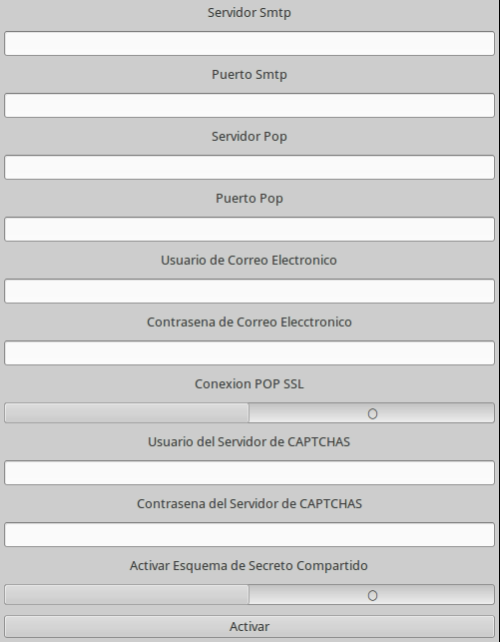
\includegraphics[width=5cm, height=5cm]{./images/VentanaConfig.png}
	\caption{Ventana de Configuración}
	\label{fig:6-10-1}
\end{figure}

Posteriormente se gener\'o una interfaz gráfica principal para visualizar los mensajes de correos electrónicos y una segunda interfaz para la redacción de los mismos.

\begin{figure}[H]
\centering
	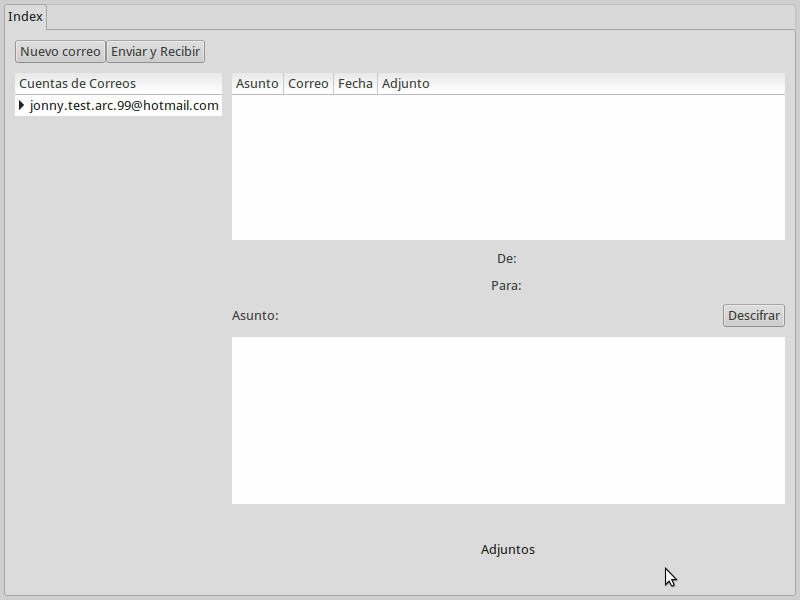
\includegraphics[width=7.5cm, height=5cm]{./images/VentanaPrincipal.png}
	\caption{Ventana Principal}
	\label{fig:6-10-2}
\end{figure}

La primera  interfaz, también llamada ventana principal, esta dividida en 3 partes: una barra lateral, un listado y un visualizador de mensajes de correo electrónico. En la barra lateral encontramos las carpetas donde se almacenan los correo electrónicos, en el listado encontramos los mensajes de correos electrónicos que se han almacenado en la carpeta seleccionada de la barra lateral y por ultimo tenemos el visualizador de mensajes, el cual  despliega la dirección de correo del usuario que mando ese mensaje, los destinatarios a donde fue dirigido el mensaje y por \'ultimo el cuerpo del mensaje, ver Figura~\ref{fig:6-10-2}.

La segunda interfaz, también llamada ventana de envío de mensajes,  tiene un diseño simple para redactar los mensajes de correo electrónico, esta interfaz cuenta con 3 espacios, el primero es para escribir la dirección de correo donde se enviará el mensaje; el segundo espacio es para escribir el asunto que se adjunta al mensaje; y por último espacio es para la redacción del mismo, ver Figura ~\ref{fig:6-10-3}.
\begin{figure}[t]
\centering
	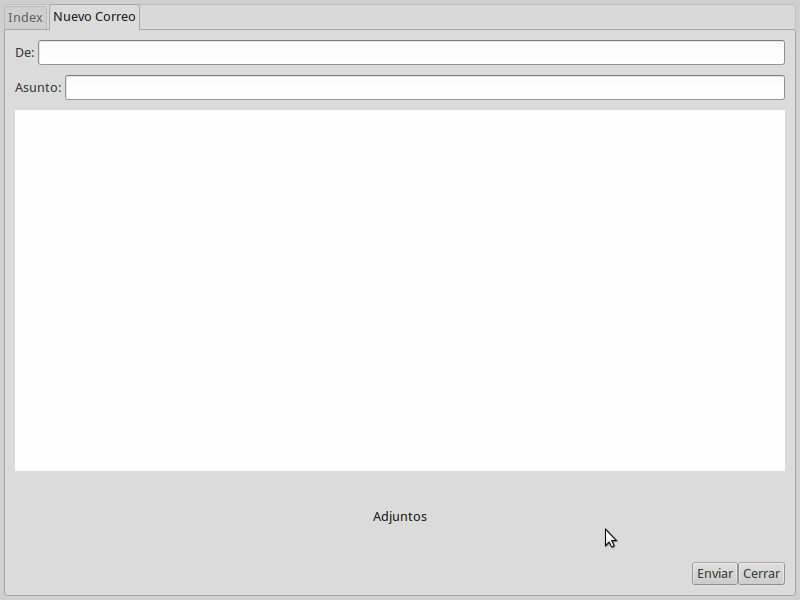
\includegraphics[width=7.5cm, height=5cm]{./images/VentanaNewCorreo.png}
	\caption{Ventana de Nuevo Correo}
	\label{fig:6-10-3}
\end{figure}
Una vez que se tienen las interfaces listas se procede a darles funcionalidad, para ello se llevaron a cabo las siguientes actividades.
\begin{itemize}
 \item Cifrado de mensajes de correo electrónico por el protocolo $\mathbb{P}$ y ${\mathbb P}^{\prime}$:
  Esta actividad se inicia al redactar un correo electrónico en la ventana de envío de mensaje y pulsar el botón enviar. 
Lo primero que hace es tomar la fecha actual de la computadora y se concatena con las dirección de correo destino y origen, a esta cadena generada  se le  obtiene un digesto MD5, el cual ser\'a utilizado como firma para el mensaje de correo. Posteriormente se toma el mensaje redactado por el usuario y es enviado a la biblioteca de cifrado, especificando el protocolo a usar. Esta biblioteca nos regresa el mensaje cifrado junto con la ruta de la imágenes CAPTCHAS que descifran el mensaje. Después se toma este mensaje cifrado y se  concatena con la firma generada anteriormente  y con una cabecera que nos indicar\'a si el mensaje esta cifrado o no al momento de visualizarlo. A continuación toma las direcciones de correo, origen y destino, el asunto redactado y el mensaje cifrado para generar un mensaje de correo electrónico y guardarlo en la carpeta de salida, éste mensaje será enviado posteriormente por el protocolo SMTP al servidor de correos. Por último esta actividad activa el envío de imágenes CAPTCHAS al servidor de CAPTCHAS.
 \item Envío de imágenes CAPTCHAS al servidor de CAPTCHAS: Esta actividad se inicia al momento de pulsar el botón “Enviar y Recibir” de la ventana principal o al termino del cifrado de mensajes de correo electrónico.
Se toma un listado de los mensajes de correo que se tienen pendientes de envío en la carpeta de salida, buscando los CAPTCHAS correspondientes a cada mensaje. Cada uno de estos CAPTCHAS son enviados al servidor junto con las direcciones de correo origen y destino, la firma del mensaje de correo y los datos de configuración del archivo JSON por medio de una petición HTTP. Por último, por cada CAPTCHA enviado exitosamente se envía su correspondiente mensaje al servidor de correo por el protocolo SMTP.
 \item Envío de mensajes por el protocolo SMTP: Esta actividad se inicia al momento de pulsar el botón “Enviar y Recibir” de la ventana principal o al termino de un envío exitoso de un CAPTCHA.
Para hacer el envío de un mensaje de correo electrónico se necesitan los datos de configuración que se tienen el el archivo JSON junto con el mensaje que se desea enviar. En caso de error el mensaje se almacena en la carpeta de salida.
\item Descargar mensajes por POP3: Esta actividad se inicia al momento de pulsar el botón “Enviar y Recibir” de la ventana principal.
Para iniciar la descarga de los mensajes de correo electrónico se toman los datos básicos del archivo JSON para establecer comunicación con el servidor. Una vez establecida la conexión el servidor de correo electrónico nos dará uno a uno los mensajes y el cliente de correo electrónico guardará cada mensaje en un archivo txt en la carpeta de entrada.

\item Descarga de imágenes CAPTCHAS del servidor de CAPTCHAS: Esta actividad se inicia al momento de pulsar el botón “Descifrar” de la ventana principal.
Para saber si el mensaje esta cifrado se busca en el cuerpo del mensaje la cabecera de cifrado de donde obtenemos la firma del mensaje. Con la firma del mensaje se buscan las imágenes de descifrado en la carpeta CAPTCHA, esta carpeta se crea con la instalación del prototipo, en caso de no encontrar las imágenes en la carpeta el cliente de correo hacer una petición HTTP al servidor de CAPTCHAS adjuntando la firma del mensaje, las direcciones de origen y la dirección destino.
El servidor contesta enviando la dirección URL de la imágenes de  donde  el cliente descarga las imágenes y las guarda en la carpeta CAPTCHA. Después de guardarlas, el cliente despliega la o las imágenes CAPTCHA en una ventana para que el usuario lo resuelva, esta ventana la llamaremos ventana de Descifrado. El despliegue de una o mas imágenes dependerá del protocolo que se haya utilizado para cifrar.
\begin{figure}[H]
\centering
	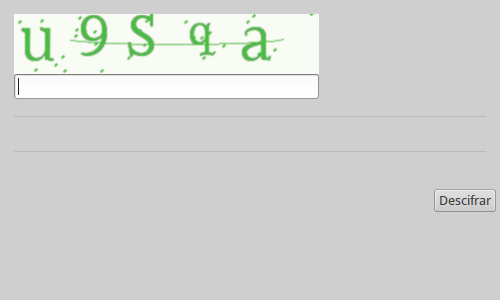
\includegraphics[width=5cm, height=2.5cm]{./images/VentanaCAPTCHA.png}
	\caption{Ventana CAPTCHAS}
	\label{fig:6-10-4}
\end{figure}
 \item Descifrado de mensajes de correo electrónico por el protocolo $\mathbb{P}$ y ${\mathbb{P}}^{\prime}$:
Esta actividad se inicia al momento de pulsar el botón “Descifrar” de la ventana de Descifrado.
Una vez que el usuario resuelve los CAPTCHAS se toman las respuestas junto con el cuerpo del mensaje cifrado sin la cabecera de cifrado y se envían a la biblioteca de cifrado,  la cual nos regresa el texto descifrado. En caso de que los CAPTCHAS sean ingresados incorrectamente el texto regresado por la biblioteca sera ilegible y el cliente de correos lo detectar\'a.
\end{itemize}
%\textbf{Conclusión:}  El cliente de correo electrónico que se describió en este prototipo es completamente funcional y en conjunto con los prototipos 8 y 9 cumplen con el funcionamiento del esquema propuesto en este documento para implementar los protocolos P y P’ del esquema Díaz -Chakraborty. Para ver el codigo completo del prototipo 10 ver el anexo 5.
\begin{figure}[H]
\centering
	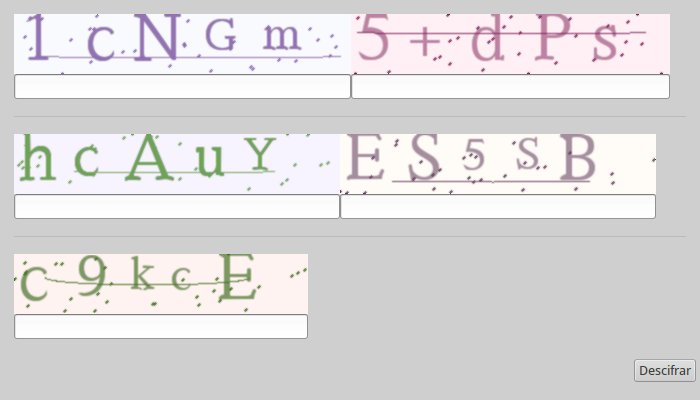
\includegraphics[width=7.5cm, height=3.5cm]{./images/VentanaMultiCAPTCHAS.png}
	\caption{Ventana Multi-CAPTCHAS}
	\label{fig:6-10-5}
\end{figure}
\section{Conclusiones}
\label{sec-conclusion}
En el desarrollo de este trabajo terminal se encontraron varios problemas al desarrollar complementos para clientes de correo electrónico comerciales los cuales describiremos a continuación.

El primer problema encontrado fue la gran cantidad de tiempo que se invierte en la investigación, desarrollo, revisión y correcciones de los complementos que se implementan para los clientes de correo estándar, ya que si se desea publicar un complemento con la empresa que desarrollo el cliente, éstos son sometido a una evaluación para verificar que no altere el funcionamiento de otros módulos de su cliente.

Otro problema a tomar en cuenta es la fase de desarrollo en la que se encuentra el cliente de correo que se desea ocupar, ya que si se encuentra en una etapa muy temprana de desarrollo se encontrara poca documentación; las funciones disponibles serán limitadas; y muy probablemente cambien la compatibilidad entre módulos de una versión a otra. 

La solución que se implement\'o fue desarrollar un cliente de correo electrónico que tuviera las funciones básicas de envío y recepción de mensajes de correo electrónico por los protocolos POP3 y SMTP, junto con la implementación de los protocolos $\mathbb{P}$ y ${\mathbb{P}}^{\prime}$ del esquema Díaz – Chakraborty para el cifrado y descifrado de los mensajes de correo electrónico por medio de CAPTCHAS.
Se observó que el intercambio de clave y la implementación de los protocolos $\mathbb{P}$ y ${\mathbb{P}}^{\prime}$ del esquema Díaz - Chakraborty se llevó con éxito. También se concluye que estos esquemas pueden implementarse en los modelos actuales de comunicación de correo electrónico de una manera trasparente al usuario al momento del envío y recepción de los correos electrónicos. Cabe destacar que es la primera implementación funcional que se tiene del esquema de secreto compartido de Adi Shamir para el correo electrónico e inhibiendo los ataques de los agentes clasificadores.

Por último se encontró que las comunicaciones que se establecen actualmente entre los servidores de correo electrónico y los usuarios son canales seguros. Lo cual fue confirmado por las pruebas realizadas a la aplicación, por lo tanto se concluye que el ataque de los adversarios clasificadores se hace en los servidores de correo electrónico donde son almacenados los mensajes en claro y se tiene acceso a un gran número de mensajes para su clasificación.

% conference papers do not normally have an appendix

% use section* for acknowledgement
%\section*{Acknowledgment}
% optional entry into table of contents (if used)
%\addcontentsline{toc}{section}{Acknowledgment}
%The authors would like to thank...

% trigger a \newpage just before the given reference
% number - used to balance the columns on the last page
% adjust value as needed - may need to be readjusted if
% the document is modified later
%\IEEEtriggeratref{8}
% The "triggered" command can be changed if desired:
%\IEEEtriggercmd{\enlargethispage{-5in}}

% references section
% NOTE: BibTeX documentation can be easily obtained at:
% http://www.ctan.org/tex-archive/biblio/bibtex/contrib/doc/

% can use a bibliography generated by BibTeX as a .bbl file
% standard IEEE bibliography style from:
% http://www.ctan.org/tex-archive/macros/latex/contrib/supported/IEEEtran/bibtex
%\bibliographystyle{IEEEtran.bst}
% argument is your BibTeX string definitions and bibliography database(s)
%\bibliography{IEEEabrv,../bib/paper}
%
% <OR> manually copy in the resultant .bbl file
% set second argument of \begin to the number of references
% (used to reserve space for the reference number labels box)
\bibliographystyle{abbrv} %{plain}
\bibliography{bibliografia}

% that's all folks
\end{document}


